\documentclass[0-protokol.tex]{subfiles}
\begin{document}

V následující tabulce jsou uvedeny hodnoty pěti měření poloměrů velké a malé cívky pomocí pásového měřidla. Hodnoty byly získány dělením naměřených průměrů, uvedených na poslední straně v záznamu z měření, dvěma. Chyba měřidla byla určena velikostí nejmenšího dílku, tedy $\SI{1}{mm}$, a dělena dvěma.
\begin{table}[H] 
\centering
\setlength{\tabcolsep}{10pt}
\begin{tabular}{
    l
    S[table-format=3.1]
    S[table-format=3.1]
    S[table-format=3.1]
    S[table-format=3.1]
    S[table-format=3.1]
    S[table-format=3.1]
    S[table-format=1.1]
    S[table-format=0.1]
} \toprule
měření         & {1}   & {2}  & {3}   & {4}   & {5}   & {průměr} & {$\sigma_\text{měř}$} & {$\sigma$} \\ \midrule
$r_V[\si{mm}]$ & 203.5 & 200. & 202.  & 203.  & 202.5 & 202.2    & 0.5                   & 0.8        \\
$r_M[\si{mm}]$ & 103.5 & 102. & 102.5 & 103.5 & 102.5 & 102.8    & 0.5                   & 0.6        \\ \bottomrule

\end{tabular} 
\caption{Hodnoty poloměrů cívek}
\label{tab:r}
\end{table}

Vzdálenost zrcátka od stupnice byla měřena pásovým měřidlem, měřidlo bylo přiloženo ke stupnici zhruba ve čtvrtině její délky, jedná se tedy o střední hodnotu nejbližšího a nejvzdálenějšího místa stupnice od zrcátka. S touto hodnotou je následně nakládáno, jako by stupnice měla kruhové zakřivení, chyba této aproximace není velká ve srovnání s chybou měřidla, která byla kvůli prohybům a nepříznivým podmínkám měření určena na $\SI{1}{cm}$.
$$ l = \SI{1.330 \pm 0.010}{m}. $$

\subsection*{Úkol 1}

Následující tabulka shrnuje naměřené a spočtené hodnoty výchylek torzního magnetometru při působení magnetického pole generovaného malou cívkou protékanou proudem $I$. Chyba délkové výchylky $x$ byla určena na $\SI{5}{mm}$, protože i přesto, že kmity magnetometru byly tlumeny lopatkou ponořenou ve vodě, se světelná značka na stupnici pohybovala. Zároveň byla výchylka citlivá na pohyb v jejím okolí. 

Úhlová výchylka byla spočtena pomocí \eqref{eq:alpha}. 
\begin{table}[H] 
\centering
\setlength{\tabcolsep}{10pt}
\begin{tabular}{
    S[table-format=1.1]
    S[table-format=2.0]
    S[table-format=1.0]
    S[table-format=0.4]
    S[table-format=0.4]
    S[table-format=3.0]
    S[table-format=1.0]
    S[table-format=0.4]
    S[table-format=0.4]
} \toprule
{$I$}        & {$x^M_{N=5}$} & {$\sigma_{x^M_{N=5}}$} & {$\alpha^M_{N=5}$} & {$\sigma_{\alpha^M_{N=5}}$} & {$x^M_{N=10}$} & {$\sigma_{x^M_{N=10}}$} & {$\alpha^M_{N=10}$} & {$\sigma_{\alpha^M_{N=10}}$} \\
{$[\si{A}]$} & {$[\si{mm}]$} & {$[\si{mm}]$}          & {$[\si{\rad}]$}    & {$[\si{\rad}]$}             & {$[\si{mm}]$}  & {$[\si{mm}]$}           & {$[\si{\rad}]$}     & {$[\si{\rad}]$}              \\ \midrule
0.0          & 000           & 5                      & 0.0000             & 0.0019                      & 000            & 5                       & 0.0000              & 0.0019                       \\
0.5          & 019           & 5                      & 0.0071             & 0.0019                      & 035            & 5                       & 0.0132              & 0.0019                       \\
1.0          & 036           & 5                      & 0.0135             & 0.0019                      & 073            & 5                       & 0.0274              & 0.0019                       \\
1.5          & 055           & 5                      & 0.0207             & 0.0019                      & 107            & 5                       & 0.0402              & 0.0019                       \\
2.0          & 072           & 5                      & 0.0271             & 0.0019                      & 145            & 5                       & 0.0545              & 0.0019                       \\
2.5          & 092           & 5                      & 0.0346             & 0.0019                      & 179            & 5                       & 0.0673              & 0.0019                       \\
3.0          & 109           & 5                      & 0.0410             & 0.0019                      & 216            & 5                       & 0.0812              & 0.0020                       \\
3.5          & 126           & 5                      & 0.0474             & 0.0019                      & 254            & 5                       & 0.0955              & 0.0020                       \\
4.0          & 144           & 5                      & 0.0541             & 0.0019                      & 291            & 5                       & 0.1094              & 0.0021                       \\ \bottomrule

\end{tabular}
\caption{Naměřené a spočtené hodnoty při použití malé cívky}
\label{tab:M}
\end{table}
\newpage
V tabulce \ref{tab:V} jsou uvedeny hodnoty stejných veličin jako výše při použití velké cívky.
\begin{table}[H] 
\centering
\setlength{\tabcolsep}{10pt}
\begin{tabular}{
    S[table-format=1.1]
    S[table-format=2.0]
    S[table-format=1.0]
    S[table-format=0.4]
    S[table-format=0.4]
    S[table-format=3.0]
    S[table-format=1.0]
    S[table-format=0.4]
    S[table-format=0.4]
} \toprule
{$I$}        & {$x^V_{N=5}$} & {$\sigma_{x^V_{N=5}}$} & {$\alpha^V_{N=5}$} & {$\sigma_{\alpha^V_{N=5}}$} & {$x^V_{N=10}$} & {$\sigma_{x^V_{N=10}}$} & {$\alpha^V_{N=10}$} & {$\sigma_{\alpha^V_{N=10}}$} \\
{$[\si{A}]$} & {$[\si{mm}]$} & {$[\si{mm}]$}          & {$[\si{\rad}]$}    & {$[\si{\rad}]$}             & {$[\si{mm}]$}  & {$[\si{mm}]$}           & {$[\si{\rad}]$}     & {$[\si{\rad}]$}              \\ \midrule
0.0          & 0             & 5                      & 0.0000             & 0.0019                      & 000            & 5                       & 0.0000              & 0.0019                       \\
0.5          & 10            & 5                      & 0.0038             & 0.0019                      & 020            & 5                       & 0.0075              & 0.0019                       \\
1.0          & 20            & 5                      & 0.0075             & 0.0019                      & 040            & 5                       & 0.0150              & 0.0019                       \\
1.5          & 29            & 5                      & 0.0109             & 0.0019                      & 058            & 5                       & 0.0218              & 0.0019                       \\
2.0          & 40            & 5                      & 0.0150             & 0.0019                      & 077            & 5                       & 0.0289              & 0.0019                       \\
2.5          & 50            & 5                      & 0.0188             & 0.0019                      & 096            & 5                       & 0.0361              & 0.0019                       \\
3.0          & 57            & 5                      & 0.0214             & 0.0019                      & 113            & 5                       & 0.0425              & 0.0019                       \\
3.5          & 65            & 5                      & 0.0244             & 0.0019                      & 133            & 5                       & 0.0500              & 0.0019                       \\
4.0          & 77            & 5                      & 0.0289             & 0.0019                      & 152            & 5                       & 0.0571              & 0.0019                       \\ \bottomrule

\end{tabular}
\caption{Naměřené a spočtené hodnoty při použití velké cívky}
\label{tab:V}
\end{table}

\subsection*{Úkol 2}

V grafech \ref{fig:M} a \ref{fig:V} jsou zaznamenány průběhy výchylky $\alpha$ na protékajícím proudu společně s regresními přímkami.

\begin{figure}[H]
\centering
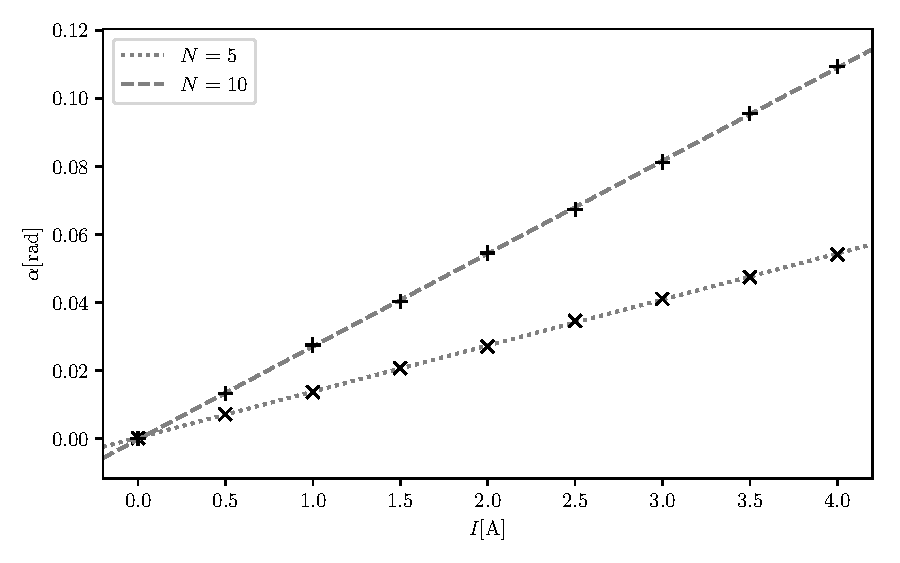
\includegraphics[]{M}
\caption{Závislost výchylky magnetometru na proudu protékajícím malou cívkou}
\label{fig:M}
\end{figure}

\begin{figure}[H]
\centering
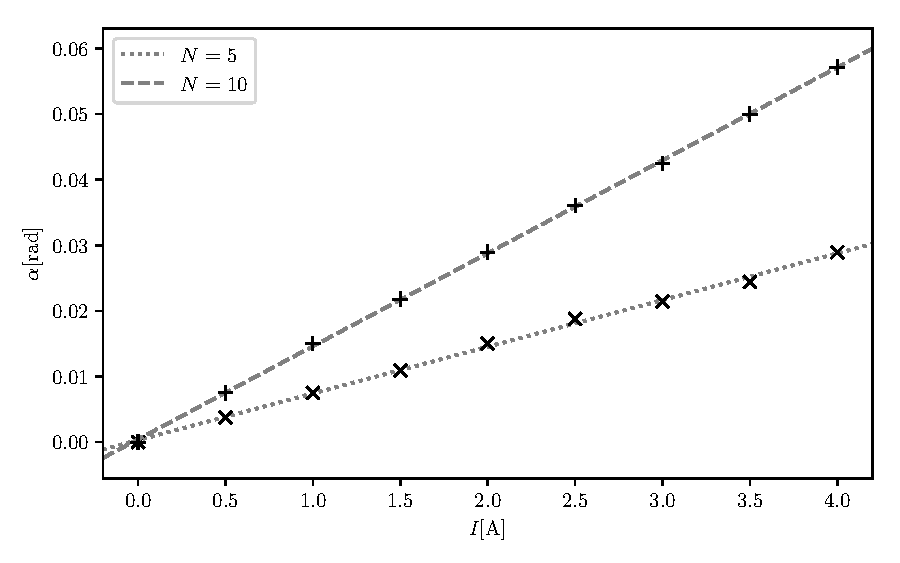
\includegraphics[]{V}
\caption{Závislost výchylky magnetometru na proudu protékajícím velkou cívkou}
\label{fig:V}
\end{figure}

Níže jsou uvedeny směrnice regresních přímek.

$$ S^M_{N=5} = \SI{1.354 \pm 0.008 e-2}{\per\ampere}, $$
$$ S^M_{N=10} = \SI{2.731 \pm 0.012 e-2}{\per\ampere}, $$
$$ S^V_{N=5} = \SI{0.712 \pm 0.012 e-2}{\per\ampere}, $$
$$ S^V_{N=10} = \SI{1.417 \pm 0.008 e-2}{\per\ampere}. $$

\subsection*{Úkol 4}

V následující tabulce lze nalézt hodoty pěti měření kmitů tozzního kyvadla, tvořeného kovovým vláknem torzního magnetometru a kovovou tyčkou o momentu setrvačnosti 
$$ J = \SI{2.72 e-4}{\kilogram\metre\squared}. $$
Měřeno bylo vždy pět kmitů, naměřené časy lze najít na poslední straně v záznamu z měření. Tabulka obsahuje periody jednoho kmitu. Chyba měření byla určena reakční schopností experimentátora jako $\SI{0.2}{s}$, následně dělena pěti.
\begin{table}[H] 
\centering
\setlength{\tabcolsep}{10pt}
\begin{tabular}{
    l
    S[table-format=1.2]
    S[table-format=1.2]
    S[table-format=1.2]
    S[table-format=1.2]
    S[table-format=1.2]
    S[table-format=1.2]
    S[table-format=1.2]
    S[table-format=1.2]
} \toprule
měření       & {1}  & {2}  & {3}  & {4}  & {5}  & {průměr} & {$\sigma_\text{měř}$} & {$\sigma$} \\ \midrule
$T[\si{mm}]$ & 4.03 & 4.05 & 4.02 & 4.03 & 4.02 & 4.03     & 0.04                  & 0.04        \\ \bottomrule

\end{tabular}
\caption{Periody kmitu torzního kyvadla}
\label{tab:T}
\end{table}

Pomocí vzorce \eqref{eq:D} byl spočten direkční moment vlákna 
$$ D = \SI{6.61 \pm 0.13 e-4}{\newton\metre}. $$

\subsection*{Úkol 5}

Pomocí vzorců \eqref{eq:p} a \eqref{eq:m} byl spočten magnetický moment použitého magnetu v Coulombových i Ampérových jednotkách
$$ p = \SI{3.71 \pm 0.08 e-7}{\weber\metre}, $$
$$ m = \SI{0.295 \pm 0.006}{\ampere\metre\squared}. $$
Pro tento výpočet byla použita směrnice závislosti výchylky na proudu tekoucím malou cívkou o deseti závitech $S^M_{N=10}$.
\end{document}
